% Options for packages loaded elsewhere
\PassOptionsToPackage{unicode}{hyperref}
\PassOptionsToPackage{hyphens}{url}
%
\documentclass[
]{article}
\usepackage{lmodern}
\usepackage{amssymb,amsmath}
\usepackage{ifxetex,ifluatex}
\ifnum 0\ifxetex 1\fi\ifluatex 1\fi=0 % if pdftex
  \usepackage[T1]{fontenc}
  \usepackage[utf8]{inputenc}
  \usepackage{textcomp} % provide euro and other symbols
\else % if luatex or xetex
  \usepackage{unicode-math}
  \defaultfontfeatures{Scale=MatchLowercase}
  \defaultfontfeatures[\rmfamily]{Ligatures=TeX,Scale=1}
\fi
% Use upquote if available, for straight quotes in verbatim environments
\IfFileExists{upquote.sty}{\usepackage{upquote}}{}
\IfFileExists{microtype.sty}{% use microtype if available
  \usepackage[]{microtype}
  \UseMicrotypeSet[protrusion]{basicmath} % disable protrusion for tt fonts
}{}
\makeatletter
\@ifundefined{KOMAClassName}{% if non-KOMA class
  \IfFileExists{parskip.sty}{%
    \usepackage{parskip}
  }{% else
    \setlength{\parindent}{0pt}
    \setlength{\parskip}{6pt plus 2pt minus 1pt}}
}{% if KOMA class
  \KOMAoptions{parskip=half}}
\makeatother
\usepackage{xcolor}
\IfFileExists{xurl.sty}{\usepackage{xurl}}{} % add URL line breaks if available
\IfFileExists{bookmark.sty}{\usepackage{bookmark}}{\usepackage{hyperref}}
\hypersetup{
  pdftitle={CSCI E-106:Assignment 5},
  hidelinks,
  pdfcreator={LaTeX via pandoc}}
\urlstyle{same} % disable monospaced font for URLs
\usepackage[margin=1in]{geometry}
\usepackage{color}
\usepackage{fancyvrb}
\newcommand{\VerbBar}{|}
\newcommand{\VERB}{\Verb[commandchars=\\\{\}]}
\DefineVerbatimEnvironment{Highlighting}{Verbatim}{commandchars=\\\{\}}
% Add ',fontsize=\small' for more characters per line
\usepackage{framed}
\definecolor{shadecolor}{RGB}{248,248,248}
\newenvironment{Shaded}{\begin{snugshade}}{\end{snugshade}}
\newcommand{\AlertTok}[1]{\textcolor[rgb]{0.94,0.16,0.16}{#1}}
\newcommand{\AnnotationTok}[1]{\textcolor[rgb]{0.56,0.35,0.01}{\textbf{\textit{#1}}}}
\newcommand{\AttributeTok}[1]{\textcolor[rgb]{0.77,0.63,0.00}{#1}}
\newcommand{\BaseNTok}[1]{\textcolor[rgb]{0.00,0.00,0.81}{#1}}
\newcommand{\BuiltInTok}[1]{#1}
\newcommand{\CharTok}[1]{\textcolor[rgb]{0.31,0.60,0.02}{#1}}
\newcommand{\CommentTok}[1]{\textcolor[rgb]{0.56,0.35,0.01}{\textit{#1}}}
\newcommand{\CommentVarTok}[1]{\textcolor[rgb]{0.56,0.35,0.01}{\textbf{\textit{#1}}}}
\newcommand{\ConstantTok}[1]{\textcolor[rgb]{0.00,0.00,0.00}{#1}}
\newcommand{\ControlFlowTok}[1]{\textcolor[rgb]{0.13,0.29,0.53}{\textbf{#1}}}
\newcommand{\DataTypeTok}[1]{\textcolor[rgb]{0.13,0.29,0.53}{#1}}
\newcommand{\DecValTok}[1]{\textcolor[rgb]{0.00,0.00,0.81}{#1}}
\newcommand{\DocumentationTok}[1]{\textcolor[rgb]{0.56,0.35,0.01}{\textbf{\textit{#1}}}}
\newcommand{\ErrorTok}[1]{\textcolor[rgb]{0.64,0.00,0.00}{\textbf{#1}}}
\newcommand{\ExtensionTok}[1]{#1}
\newcommand{\FloatTok}[1]{\textcolor[rgb]{0.00,0.00,0.81}{#1}}
\newcommand{\FunctionTok}[1]{\textcolor[rgb]{0.00,0.00,0.00}{#1}}
\newcommand{\ImportTok}[1]{#1}
\newcommand{\InformationTok}[1]{\textcolor[rgb]{0.56,0.35,0.01}{\textbf{\textit{#1}}}}
\newcommand{\KeywordTok}[1]{\textcolor[rgb]{0.13,0.29,0.53}{\textbf{#1}}}
\newcommand{\NormalTok}[1]{#1}
\newcommand{\OperatorTok}[1]{\textcolor[rgb]{0.81,0.36,0.00}{\textbf{#1}}}
\newcommand{\OtherTok}[1]{\textcolor[rgb]{0.56,0.35,0.01}{#1}}
\newcommand{\PreprocessorTok}[1]{\textcolor[rgb]{0.56,0.35,0.01}{\textit{#1}}}
\newcommand{\RegionMarkerTok}[1]{#1}
\newcommand{\SpecialCharTok}[1]{\textcolor[rgb]{0.00,0.00,0.00}{#1}}
\newcommand{\SpecialStringTok}[1]{\textcolor[rgb]{0.31,0.60,0.02}{#1}}
\newcommand{\StringTok}[1]{\textcolor[rgb]{0.31,0.60,0.02}{#1}}
\newcommand{\VariableTok}[1]{\textcolor[rgb]{0.00,0.00,0.00}{#1}}
\newcommand{\VerbatimStringTok}[1]{\textcolor[rgb]{0.31,0.60,0.02}{#1}}
\newcommand{\WarningTok}[1]{\textcolor[rgb]{0.56,0.35,0.01}{\textbf{\textit{#1}}}}
\usepackage{graphicx,grffile}
\makeatletter
\def\maxwidth{\ifdim\Gin@nat@width>\linewidth\linewidth\else\Gin@nat@width\fi}
\def\maxheight{\ifdim\Gin@nat@height>\textheight\textheight\else\Gin@nat@height\fi}
\makeatother
% Scale images if necessary, so that they will not overflow the page
% margins by default, and it is still possible to overwrite the defaults
% using explicit options in \includegraphics[width, height, ...]{}
\setkeys{Gin}{width=\maxwidth,height=\maxheight,keepaspectratio}
% Set default figure placement to htbp
\makeatletter
\def\fps@figure{htbp}
\makeatother
\setlength{\emergencystretch}{3em} % prevent overfull lines
\providecommand{\tightlist}{%
  \setlength{\itemsep}{0pt}\setlength{\parskip}{0pt}}
\setcounter{secnumdepth}{-\maxdimen} % remove section numbering

\title{CSCI E-106:Assignment 5}
\author{}
\date{\vspace{-2.5em}}

\begin{document}
\maketitle

\hypertarget{due-date-october-12-2020-at-720-pm-est}{%
\subsubsection{Due Date: October 12, 2020 at 7:20 pm
EST}\label{due-date-october-12-2020-at-720-pm-est}}

\hypertarget{instructions}{%
\subsubsection{Instructions}\label{instructions}}

Students should submit their reports on Canvas. The report needs to
clearly state what question is being solved, step-by-step walk-through
solutions, and final answers clearly indicated. Please solve by hand
where appropriate.

Please submit two files: (1) a R Markdown file (.Rmd extension) and (2)
a PDF document, word, or html generated using knitr for the .Rmd file
submitted in (1) where appropriate. Please, use RStudio Cloud for your
solutions.

\begin{center}\rule{0.5\linewidth}{0.5pt}\end{center}

\hypertarget{problem-1}{%
\subsection{Problem 1}\label{problem-1}}

Refer to Plastic hardness data set. X is the elapsed time in hours? and
Y is hardness in Brinell units. Build a model to predict Y. (30 points,
5 points each)

a-) Obtain the residuals ei and prepare a box plot of the residuals.
What information is provided by your plot?

\begin{Shaded}
\begin{Highlighting}[]
\KeywordTok{rm}\NormalTok{(}\DataTypeTok{list =} \KeywordTok{ls}\NormalTok{())}

\KeywordTok{library}\NormalTok{(knitr)}
\KeywordTok{library}\NormalTok{(olsrr)}
\end{Highlighting}
\end{Shaded}

\begin{verbatim}
## 
## Attaching package: 'olsrr'
\end{verbatim}

\begin{verbatim}
## The following object is masked from 'package:datasets':
## 
##     rivers
\end{verbatim}

\begin{Shaded}
\begin{Highlighting}[]
\KeywordTok{library}\NormalTok{(onewaytests)}
\KeywordTok{library}\NormalTok{(lmtest)}
\end{Highlighting}
\end{Shaded}

\begin{verbatim}
## Loading required package: zoo
\end{verbatim}

\begin{verbatim}
## 
## Attaching package: 'zoo'
\end{verbatim}

\begin{verbatim}
## The following objects are masked from 'package:base':
## 
##     as.Date, as.Date.numeric
\end{verbatim}

\begin{Shaded}
\begin{Highlighting}[]
\KeywordTok{setwd}\NormalTok{(}\StringTok{"~/OneDrive/courses/e106/HW/HW5"}\NormalTok{) }\CommentTok{# replace with working directory of machine where this is run}
\NormalTok{plastic <-}\StringTok{ }\KeywordTok{read.csv}\NormalTok{(}\StringTok{'Plastic Hardness Data-1.csv'}\NormalTok{)}
\KeywordTok{head}\NormalTok{(plastic)}
\end{Highlighting}
\end{Shaded}

\begin{verbatim}
##     Y  X
## 1 199 16
## 2 205 16
## 3 196 16
## 4 200 16
## 5 218 24
## 6 220 24
\end{verbatim}

\begin{Shaded}
\begin{Highlighting}[]
\CommentTok{# build regression and plot residuals}
\NormalTok{reg_p1 <-}\StringTok{ }\KeywordTok{lm}\NormalTok{(plastic}\OperatorTok{$}\NormalTok{Y}\OperatorTok{~}\NormalTok{plastic}\OperatorTok{$}\NormalTok{X)}
\KeywordTok{summary}\NormalTok{(reg_p1)}
\end{Highlighting}
\end{Shaded}

\begin{verbatim}
## 
## Call:
## lm(formula = plastic$Y ~ plastic$X)
## 
## Residuals:
##     Min      1Q  Median      3Q     Max 
## -5.1500 -2.2188  0.1625  2.6875  5.5750 
## 
## Coefficients:
##              Estimate Std. Error t value Pr(>|t|)    
## (Intercept) 168.60000    2.65702   63.45  < 2e-16 ***
## plastic$X     2.03438    0.09039   22.51 2.16e-12 ***
## ---
## Signif. codes:  0 '***' 0.001 '**' 0.01 '*' 0.05 '.' 0.1 ' ' 1
## 
## Residual standard error: 3.234 on 14 degrees of freedom
## Multiple R-squared:  0.9731, Adjusted R-squared:  0.9712 
## F-statistic: 506.5 on 1 and 14 DF,  p-value: 2.159e-12
\end{verbatim}

\begin{Shaded}
\begin{Highlighting}[]
\NormalTok{ei_p1 <-}\StringTok{ }\NormalTok{reg_p1}\OperatorTok{$}\NormalTok{residuals}
\KeywordTok{boxplot}\NormalTok{(ei_p1, }\DataTypeTok{horizontal =} \OtherTok{TRUE}\NormalTok{, }\DataTypeTok{staplewax =} \FloatTok{0.5}\NormalTok{, }\DataTypeTok{col =} \DecValTok{3}\NormalTok{, }\DataTypeTok{xlab =} \StringTok{'Residuals'}\NormalTok{)}
\end{Highlighting}
\end{Shaded}

\includegraphics{homework5_files/figure-latex/unnamed-chunk-1-1.pdf}

\begin{Shaded}
\begin{Highlighting}[]
\CommentTok{#ols_plot_resid_box(reg_p1)}
\end{Highlighting}
\end{Shaded}

The boxplot appears to be symmetrical with no outliers and indicates
that there are no outliers and that the error terms are normally
distributed.

b-) Plot the residuals ei against the fitted values Y; to ascertain
whether any departures from regression model (2.1) are evident. State
your findings.

\begin{Shaded}
\begin{Highlighting}[]
\CommentTok{#ols_plot_resid_fit(reg_p1)}
\NormalTok{old.par <-}\StringTok{ }\KeywordTok{par}\NormalTok{(}\DataTypeTok{mfrow =} \KeywordTok{c}\NormalTok{(}\DecValTok{2}\NormalTok{,}\DecValTok{2}\NormalTok{))}
\KeywordTok{plot}\NormalTok{(reg_p1)}
\end{Highlighting}
\end{Shaded}

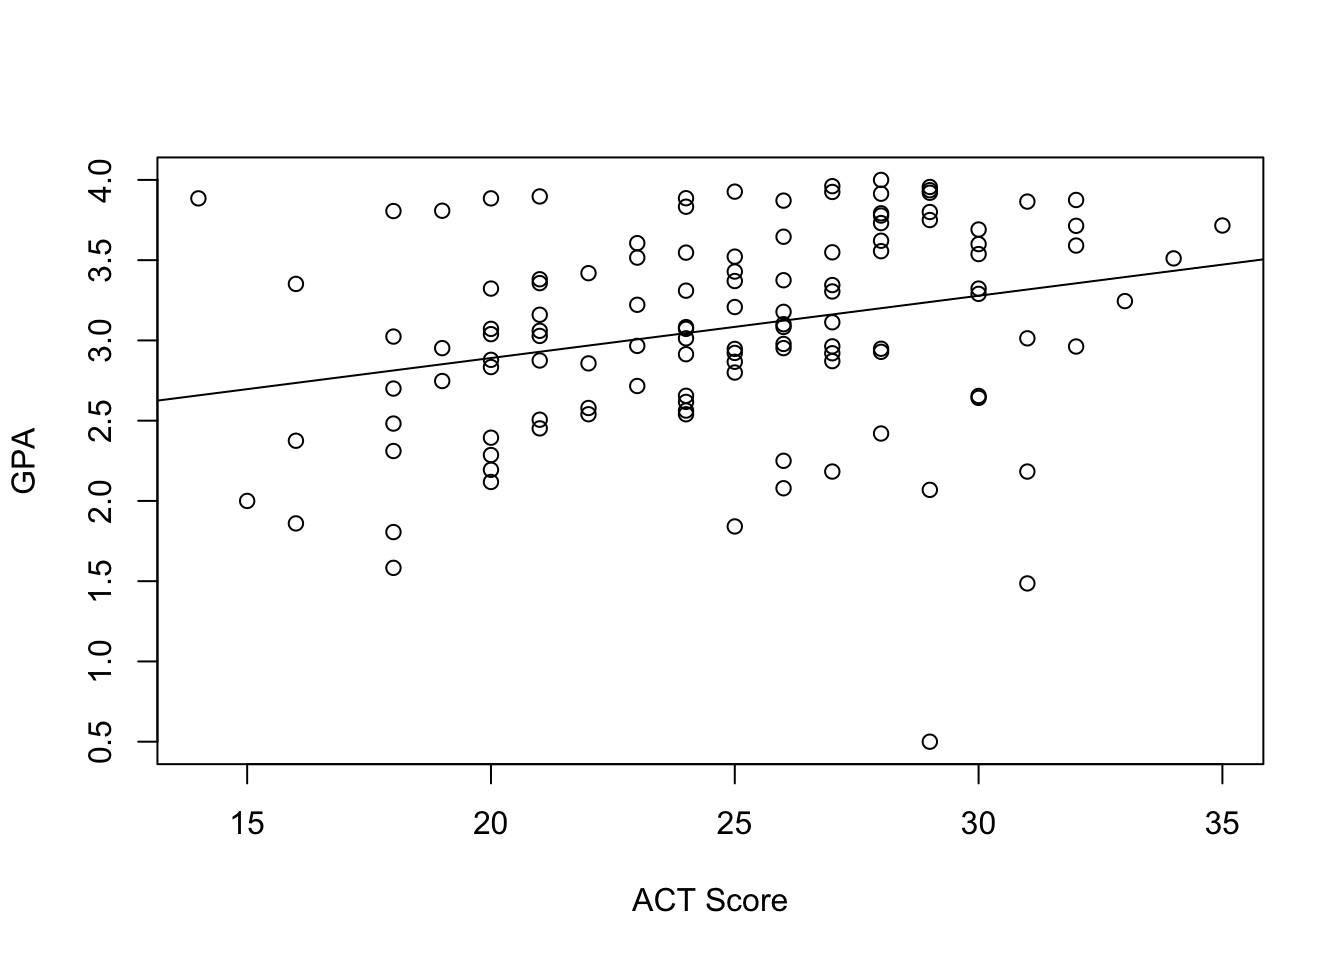
\includegraphics{homework5_files/figure-latex/unnamed-chunk-2-1.pdf}

\begin{Shaded}
\begin{Highlighting}[]
\NormalTok{old.par}
\end{Highlighting}
\end{Shaded}

\begin{verbatim}
## $mfrow
## [1] 1 1
\end{verbatim}

The residual vs fitted values plot indicates the presence of outliers as
well as a pattern in the distribution. This means that regression
assumptions are not satisfied.

c-) Prepare a normal probability plot of the residuals. Also obtain the
coefficient of correlation between the ordered residuals and their
expected values under normality. Does the normality assumption appear to
be reasonable here?

\begin{Shaded}
\begin{Highlighting}[]
\KeywordTok{ols_plot_resid_qq}\NormalTok{(reg_p1)}
\end{Highlighting}
\end{Shaded}

\includegraphics{homework5_files/figure-latex/unnamed-chunk-3-1.pdf}

\begin{Shaded}
\begin{Highlighting}[]
\KeywordTok{ols_test_correlation}\NormalTok{(reg_p1)}
\end{Highlighting}
\end{Shaded}

\begin{verbatim}
## [1] 0.9916733
\end{verbatim}

The residual values are highly correlated with their expected values
under normality as seen from the correlation values. However, this is
only within the range of 1-SD while the values diverge beyond this.

The line also does not appear to be at 45 degrees as should be for the
condiiton to be satisfied.

d-) Compare the frequencies of the residuals against the expected
frequencies under normality, using the 25th, 50th, and 75th percentiles
of the relevant t distribution. Is the information provided by these
comparisons consistent with the findings from the normal probability
plot in part (c)?

As seen from the plot in 1(c) above, the x-axis denotes the theoretical
quantiles.

0 value on x-axis corresponds to 50th percentile and we see that equal
number of points are to the left and right of it

-1 value on x-axis corresponds approxmately to 25th percentile while +1
value on x-axis corresponds to 75th percentile.

We see from the plot that 10 points out of total 16, i.e.~62\% fall
within the range of + or - 1SD. This is close to the expected 68\% and
may converge with higher values.

e-) Use the Brown-Forsythe test to determine whether or not the error
variance varies with the level of X. Divide the data into the two
groups, X \(\leq\) 24, X \textgreater{} 24, and use \(\alpha=0.01\).
State the decision rule and conclusion. Does your conclusion support
your preliminary findings in part (b)?

\begin{Shaded}
\begin{Highlighting}[]
\NormalTok{bf.data <-}\StringTok{ }\KeywordTok{data.frame}\NormalTok{(}\KeywordTok{cbind}\NormalTok{(plastic, reg_p1}\OperatorTok{$}\NormalTok{residuals, reg_p1}\OperatorTok{$}\NormalTok{fitted.values))}

\KeywordTok{dimnames}\NormalTok{(bf.data) }\CommentTok{# all dim names}
\end{Highlighting}
\end{Shaded}

\begin{verbatim}
## [[1]]
##  [1] "1"  "2"  "3"  "4"  "5"  "6"  "7"  "8"  "9"  "10" "11" "12" "13" "14" "15"
## [16] "16"
## 
## [[2]]
## [1] "Y"                    "X"                    "reg_p1.residuals"    
## [4] "reg_p1.fitted.values"
\end{verbatim}

\begin{Shaded}
\begin{Highlighting}[]
\KeywordTok{dim}\NormalTok{(bf.data)}
\end{Highlighting}
\end{Shaded}

\begin{verbatim}
## [1] 16  4
\end{verbatim}

\begin{Shaded}
\begin{Highlighting}[]
\KeywordTok{dimnames}\NormalTok{(bf.data)[[}\DecValTok{2}\NormalTok{]][}\DecValTok{3}\OperatorTok{:}\DecValTok{4}\NormalTok{] <-}\StringTok{ }\KeywordTok{c}\NormalTok{(}\StringTok{'residuals'}\NormalTok{, }\StringTok{'fitted.values'}\NormalTok{)}

\NormalTok{bf.data1 <-}\StringTok{ }\KeywordTok{data.frame}\NormalTok{(}\KeywordTok{cbind}\NormalTok{(bf.data, }\DataTypeTok{ind =} \KeywordTok{as.factor}\NormalTok{(}\KeywordTok{I}\NormalTok{(bf.data}\OperatorTok{$}\NormalTok{X}\OperatorTok{<=}\KeywordTok{median}\NormalTok{(bf.data}\OperatorTok{$}\NormalTok{X))}\OperatorTok{*}\DecValTok{1}\NormalTok{)))}
\KeywordTok{dim}\NormalTok{(bf.data1) }\CommentTok{# confirm Indicator column added at end}
\end{Highlighting}
\end{Shaded}

\begin{verbatim}
## [1] 16  5
\end{verbatim}

\begin{Shaded}
\begin{Highlighting}[]
\KeywordTok{bf.test}\NormalTok{(residuals}\OperatorTok{~}\NormalTok{ind, }\DataTypeTok{data =}\NormalTok{ bf.data1)}
\end{Highlighting}
\end{Shaded}

\begin{verbatim}
## 
##   Brown-Forsythe Test (alpha = 0.05) 
## ------------------------------------------------------------- 
##   data : residuals and ind 
## 
##   statistic  : 0.06942228 
##   num df     : 1 
##   denom df   : 13.1945 
##   p.value    : 0.7962498 
## 
##   Result     : Difference is not statistically significant. 
## -------------------------------------------------------------
\end{verbatim}

Decision rule for the B-F test is

H\_o : Errors are normally distributed. H\_a : Errors are not normally
distributed.

In above case the p-value is 0.7962498 wich is greater than 0.05 and
hence we fail to reject the Null hypothesis and conclude that errors are
normally distributed.

f-) conduct the Breusch-Pagan test to determine whether or not the error
variance varies with the level of X. Use \(\alpha=0.01\). State the
alternatives. decision rule, and conclusion. Is your conclusion
consistent with your preliminary findings in part (b)?

\begin{Shaded}
\begin{Highlighting}[]
\KeywordTok{bptest}\NormalTok{(reg_p1)}
\end{Highlighting}
\end{Shaded}

\begin{verbatim}
## 
##  studentized Breusch-Pagan test
## 
## data:  reg_p1
## BP = 0.8118, df = 1, p-value = 0.3676
\end{verbatim}

Decision rule for B-P test is

H\_o : Errors are normally distributed. H\_a : Errors are not normally
distributed.

In above case the p-value is 0.8118 which is greater than 0.01 and hence
we fail to reject the Null hypothesis and conclude that errors are
normally distributed.

\hypertarget{problem-2}{%
\subsection{Problem 2}\label{problem-2}}

Refer to Sales growth Data. (30 points, 10 points each)

a-) Divide the range of the predictor variable (coded years) into five
bands of width 2.0, as follows: Band 1 ranges from X = -.5 to X = 1.5;
band 2 ranges from X = 1.5 to X = 3.5; and so on. Determine the median
value of X and the median value of Y in each band and develop the band
smooth by connecting the five pairs of medians by straight lines on a
scatter plot of the data. Does the band smooth suggest that the
regression relation is linear? Discuss.

\begin{Shaded}
\begin{Highlighting}[]
\NormalTok{sales <-}\StringTok{ }\KeywordTok{read.csv}\NormalTok{(}\StringTok{'Sales Growth Data.csv'}\NormalTok{)}
\KeywordTok{head}\NormalTok{(sales)}
\end{Highlighting}
\end{Shaded}

\begin{verbatim}
##     Y X
## 1  98 0
## 2 135 1
## 3 162 2
## 4 178 3
## 5 221 4
## 6 232 5
\end{verbatim}

\begin{Shaded}
\begin{Highlighting}[]
\KeywordTok{dim}\NormalTok{(sales)}
\end{Highlighting}
\end{Shaded}

\begin{verbatim}
## [1] 10  2
\end{verbatim}

\begin{Shaded}
\begin{Highlighting}[]
\KeywordTok{plot}\NormalTok{(sales}\OperatorTok{$}\NormalTok{X, sales}\OperatorTok{$}\NormalTok{Y)}
\end{Highlighting}
\end{Shaded}

\includegraphics{homework5_files/figure-latex/unnamed-chunk-6-1.pdf}

\begin{Shaded}
\begin{Highlighting}[]
\NormalTok{sales1 <-}\StringTok{ }\KeywordTok{subset}\NormalTok{(sales, X}\OperatorTok{>-}\FloatTok{0.5} \OperatorTok{&}\StringTok{ }\NormalTok{X}\OperatorTok{<}\FloatTok{1.5}\NormalTok{)}
\NormalTok{sales2 <-}\StringTok{ }\KeywordTok{subset}\NormalTok{(sales, X}\OperatorTok{>}\FloatTok{1.5} \OperatorTok{&}\StringTok{ }\NormalTok{X}\OperatorTok{<}\FloatTok{3.5}\NormalTok{)}
\NormalTok{sales3 <-}\StringTok{ }\KeywordTok{subset}\NormalTok{(sales, X}\OperatorTok{>}\FloatTok{3.5} \OperatorTok{&}\StringTok{ }\NormalTok{X}\OperatorTok{<}\FloatTok{5.5}\NormalTok{)}
\NormalTok{sales4 <-}\StringTok{ }\KeywordTok{subset}\NormalTok{(sales, X}\OperatorTok{>}\FloatTok{5.5} \OperatorTok{&}\StringTok{ }\NormalTok{X}\OperatorTok{<}\FloatTok{7.5}\NormalTok{)}
\NormalTok{sales5 <-}\StringTok{ }\KeywordTok{subset}\NormalTok{(sales, X}\OperatorTok{>}\FloatTok{7.5} \OperatorTok{&}\StringTok{ }\NormalTok{X}\OperatorTok{<}\FloatTok{9.5}\NormalTok{)}

\NormalTok{s1x <-}\StringTok{ }\KeywordTok{median}\NormalTok{(sales1}\OperatorTok{$}\NormalTok{X)}
\NormalTok{s1y <-}\StringTok{ }\KeywordTok{median}\NormalTok{(sales1}\OperatorTok{$}\NormalTok{Y)}

\NormalTok{s2x <-}\StringTok{ }\KeywordTok{median}\NormalTok{(sales2}\OperatorTok{$}\NormalTok{X)}
\NormalTok{s2y <-}\StringTok{ }\KeywordTok{median}\NormalTok{(sales2}\OperatorTok{$}\NormalTok{Y)}

\NormalTok{s3x <-}\StringTok{ }\KeywordTok{median}\NormalTok{(sales3}\OperatorTok{$}\NormalTok{X)}
\NormalTok{s3y <-}\StringTok{ }\KeywordTok{median}\NormalTok{(sales3}\OperatorTok{$}\NormalTok{Y)}

\NormalTok{s4x <-}\StringTok{ }\KeywordTok{median}\NormalTok{(sales4}\OperatorTok{$}\NormalTok{X)}
\NormalTok{s4y <-}\StringTok{ }\KeywordTok{median}\NormalTok{(sales4}\OperatorTok{$}\NormalTok{Y)}

\NormalTok{s5x <-}\StringTok{ }\KeywordTok{median}\NormalTok{(sales5}\OperatorTok{$}\NormalTok{X)}
\NormalTok{s5y <-}\StringTok{ }\KeywordTok{median}\NormalTok{(sales5}\OperatorTok{$}\NormalTok{Y)}

\NormalTok{med_x <-}\StringTok{ }\KeywordTok{c}\NormalTok{(s1x, s2x, s3x, s4x, s5x)}
\NormalTok{med_y <-}\StringTok{ }\KeywordTok{c}\NormalTok{(s1y, s2y, s3y, s4y, s5y)}

\KeywordTok{plot}\NormalTok{(med_x, med_y, }\DataTypeTok{type =} \StringTok{'b'}\NormalTok{, }\DataTypeTok{xlab =} \StringTok{'Median of X'}\NormalTok{, }\DataTypeTok{ylab =} \StringTok{'Median of Y'}\NormalTok{, }\DataTypeTok{col =} \StringTok{'red'}\NormalTok{)}
\end{Highlighting}
\end{Shaded}

\includegraphics{homework5_files/figure-latex/unnamed-chunk-6-2.pdf} The
plot suggests that the regression is linear for lower values but turns
towards non-linearity for higher values.

b-) Create a series of seven overlapping neighborhoods of width 3.0
beginning at X = -.5. The first neighborhood will range from X = -.5 to
X = 2.5; the second neighborhood will range from X = .5 to X = 3.5; and
so on. For each of the seven overlapping neighborhoods, fit a linear
regression function and obtain the fitted value \(\hat{Y_{c}}\) at the
center \(X_{c}\) of the neighborhood. Develop a simplified version of
the lowess smooth by connecting the seven (\(X_c\), \(\hat{Y_{c}}\))
pairs by straight lines on a scatter plot of the data.

\begin{Shaded}
\begin{Highlighting}[]
\NormalTok{sales21 <-}\StringTok{ }\KeywordTok{subset}\NormalTok{(sales, X}\OperatorTok{>-}\FloatTok{0.5} \OperatorTok{&}\StringTok{ }\NormalTok{X}\OperatorTok{<}\FloatTok{2.5}\NormalTok{)}
\NormalTok{sales22 <-}\StringTok{ }\KeywordTok{subset}\NormalTok{(sales, X}\OperatorTok{>}\FloatTok{0.5} \OperatorTok{&}\StringTok{ }\NormalTok{X}\OperatorTok{<}\FloatTok{3.5}\NormalTok{)}
\NormalTok{sales23 <-}\StringTok{ }\KeywordTok{subset}\NormalTok{(sales, X}\OperatorTok{>}\FloatTok{1.5} \OperatorTok{&}\StringTok{ }\NormalTok{X}\OperatorTok{<}\FloatTok{4.5}\NormalTok{)}
\NormalTok{sales24 <-}\StringTok{ }\KeywordTok{subset}\NormalTok{(sales, X}\OperatorTok{>}\FloatTok{2.5} \OperatorTok{&}\StringTok{ }\NormalTok{X}\OperatorTok{<}\FloatTok{5.5}\NormalTok{)}
\NormalTok{sales25 <-}\StringTok{ }\KeywordTok{subset}\NormalTok{(sales, X}\OperatorTok{>}\FloatTok{3.5} \OperatorTok{&}\StringTok{ }\NormalTok{X}\OperatorTok{<}\FloatTok{6.5}\NormalTok{)}
\NormalTok{sales26 <-}\StringTok{ }\KeywordTok{subset}\NormalTok{(sales, X}\OperatorTok{>}\FloatTok{4.5} \OperatorTok{&}\StringTok{ }\NormalTok{X}\OperatorTok{<}\FloatTok{7.5}\NormalTok{)}
\NormalTok{sales27 <-}\StringTok{ }\KeywordTok{subset}\NormalTok{(sales, X}\OperatorTok{>}\FloatTok{5.5} \OperatorTok{&}\StringTok{ }\NormalTok{X}\OperatorTok{<}\FloatTok{8.5}\NormalTok{)}

\NormalTok{x21 <-}\StringTok{ }\KeywordTok{median}\NormalTok{(sales21}\OperatorTok{$}\NormalTok{X)}
\NormalTok{x22 <-}\StringTok{ }\KeywordTok{median}\NormalTok{(sales22}\OperatorTok{$}\NormalTok{X)}
\NormalTok{x23 <-}\StringTok{ }\KeywordTok{median}\NormalTok{(sales23}\OperatorTok{$}\NormalTok{X)}
\NormalTok{x24 <-}\StringTok{ }\KeywordTok{median}\NormalTok{(sales24}\OperatorTok{$}\NormalTok{X)}
\NormalTok{x25 <-}\StringTok{ }\KeywordTok{median}\NormalTok{(sales25}\OperatorTok{$}\NormalTok{X)}
\NormalTok{x26 <-}\StringTok{ }\KeywordTok{median}\NormalTok{(sales26}\OperatorTok{$}\NormalTok{X)}
\NormalTok{x27 <-}\StringTok{ }\KeywordTok{median}\NormalTok{(sales27}\OperatorTok{$}\NormalTok{X)}

\NormalTok{reg21 <-}\StringTok{ }\KeywordTok{lm}\NormalTok{(Y}\OperatorTok{~}\NormalTok{X, }\DataTypeTok{data =}\NormalTok{ sales21)}
\NormalTok{reg22 <-}\StringTok{ }\KeywordTok{lm}\NormalTok{(Y}\OperatorTok{~}\NormalTok{X, }\DataTypeTok{data =}\NormalTok{ sales22)}
\NormalTok{reg23 <-}\StringTok{ }\KeywordTok{lm}\NormalTok{(Y}\OperatorTok{~}\NormalTok{X, }\DataTypeTok{data =}\NormalTok{ sales23)}
\NormalTok{reg24 <-}\StringTok{ }\KeywordTok{lm}\NormalTok{(Y}\OperatorTok{~}\NormalTok{X, }\DataTypeTok{data =}\NormalTok{ sales24)}
\NormalTok{reg25 <-}\StringTok{ }\KeywordTok{lm}\NormalTok{(Y}\OperatorTok{~}\NormalTok{X, }\DataTypeTok{data =}\NormalTok{ sales25)}
\NormalTok{reg26 <-}\StringTok{ }\KeywordTok{lm}\NormalTok{(Y}\OperatorTok{~}\NormalTok{X, }\DataTypeTok{data =}\NormalTok{ sales26)}
\NormalTok{reg27 <-}\StringTok{ }\KeywordTok{lm}\NormalTok{(Y}\OperatorTok{~}\NormalTok{X, }\DataTypeTok{data =}\NormalTok{ sales27)}

\NormalTok{yh_}\DecValTok{21}\NormalTok{ <-}\StringTok{ }\KeywordTok{predict}\NormalTok{(reg21, }\KeywordTok{data.frame}\NormalTok{(}\DataTypeTok{X=}\NormalTok{x21))}
\NormalTok{yh_}\DecValTok{22}\NormalTok{ <-}\StringTok{ }\KeywordTok{predict}\NormalTok{(reg22, }\KeywordTok{data.frame}\NormalTok{(}\DataTypeTok{X=}\NormalTok{x22))}
\NormalTok{yh_}\DecValTok{23}\NormalTok{ <-}\StringTok{ }\KeywordTok{predict}\NormalTok{(reg23, }\KeywordTok{data.frame}\NormalTok{(}\DataTypeTok{X=}\NormalTok{x23))}
\NormalTok{yh_}\DecValTok{24}\NormalTok{ <-}\StringTok{ }\KeywordTok{predict}\NormalTok{(reg24, }\KeywordTok{data.frame}\NormalTok{(}\DataTypeTok{X=}\NormalTok{x24))}
\NormalTok{yh_}\DecValTok{25}\NormalTok{ <-}\StringTok{ }\KeywordTok{predict}\NormalTok{(reg25, }\KeywordTok{data.frame}\NormalTok{(}\DataTypeTok{X=}\NormalTok{x25))}
\NormalTok{yh_}\DecValTok{26}\NormalTok{ <-}\StringTok{ }\KeywordTok{predict}\NormalTok{(reg26, }\KeywordTok{data.frame}\NormalTok{(}\DataTypeTok{X=}\NormalTok{x26))}
\NormalTok{yh_}\DecValTok{27}\NormalTok{ <-}\StringTok{ }\KeywordTok{predict}\NormalTok{(reg27, }\KeywordTok{data.frame}\NormalTok{(}\DataTypeTok{X=}\NormalTok{x27))}

\NormalTok{x2_med <-}\StringTok{ }\KeywordTok{c}\NormalTok{(x21, x22, x23, x24, x25, x26, x27)}
\NormalTok{yh_}\DecValTok{2}\NormalTok{ <-}\StringTok{ }\KeywordTok{c}\NormalTok{(yh_}\DecValTok{21}\NormalTok{, yh_}\DecValTok{22}\NormalTok{, yh_}\DecValTok{23}\NormalTok{, yh_}\DecValTok{24}\NormalTok{,yh_}\DecValTok{25}\NormalTok{, yh_}\DecValTok{26}\NormalTok{,yh_}\DecValTok{27}\NormalTok{)}

\KeywordTok{plot}\NormalTok{(x2_med, yh_}\DecValTok{2}\NormalTok{, }\DataTypeTok{type =} \StringTok{'b'}\NormalTok{, }\DataTypeTok{col =} \StringTok{'red'}\NormalTok{)}
\end{Highlighting}
\end{Shaded}

\includegraphics{homework5_files/figure-latex/unnamed-chunk-7-1.pdf}

c-) Obtain the 95 percent confidence band for the true regression line
and plot it on the plot prepared in part (b). Does the simplified lowess
smooth fall entirely within the confidence band for the regression line?
What does this tell you about the appropriateness of the linear
regression function?

\begin{Shaded}
\begin{Highlighting}[]
\NormalTok{reg_yh <-}\StringTok{ }\KeywordTok{lm}\NormalTok{(sales}\OperatorTok{$}\NormalTok{Y}\OperatorTok{~}\NormalTok{sales}\OperatorTok{$}\NormalTok{X)}
\NormalTok{fit_yh <-}\StringTok{ }\KeywordTok{predict}\NormalTok{(reg_yh, }\KeywordTok{data.frame}\NormalTok{(}\DataTypeTok{X =}\NormalTok{ sales}\OperatorTok{$}\NormalTok{X), }\DataTypeTok{interval =} \StringTok{'confidence'}\NormalTok{, }\DataTypeTok{level =} \FloatTok{0.95}\NormalTok{)}

\KeywordTok{plot}\NormalTok{(sales}\OperatorTok{$}\NormalTok{X, sales}\OperatorTok{$}\NormalTok{Y, }\DataTypeTok{type =} \StringTok{'p'}\NormalTok{, }\DataTypeTok{col =} \StringTok{'green'}\NormalTok{, }\DataTypeTok{xlab =} \StringTok{'Year'}\NormalTok{, }\DataTypeTok{ylab =} \StringTok{'Sales'}\NormalTok{)}
\KeywordTok{lines}\NormalTok{(x2_med, yh_}\DecValTok{2}\NormalTok{, }\DataTypeTok{type =} \StringTok{'b'}\NormalTok{, }\DataTypeTok{xlab =} \StringTok{'Median of X'}\NormalTok{, }\DataTypeTok{ylab =} \StringTok{'Median of Y'}\NormalTok{, }\DataTypeTok{col =} \StringTok{'red'}\NormalTok{)}
\KeywordTok{lines}\NormalTok{(x2_med, fit_yh[}\DecValTok{1}\OperatorTok{:}\DecValTok{7}\NormalTok{,}\DecValTok{2}\NormalTok{], }\DataTypeTok{lty =} \StringTok{'dashed'}\NormalTok{, }\DataTypeTok{col =} \StringTok{'blue'}\NormalTok{)}
\KeywordTok{lines}\NormalTok{(x2_med, fit_yh[}\DecValTok{1}\OperatorTok{:}\DecValTok{7}\NormalTok{,}\DecValTok{3}\NormalTok{], }\DataTypeTok{lty =} \StringTok{'dashed'}\NormalTok{, }\DataTypeTok{col =} \StringTok{'blue'}\NormalTok{)}
\end{Highlighting}
\end{Shaded}

\includegraphics{homework5_files/figure-latex/unnamed-chunk-8-1.pdf} The
confidence band is outside the regression line. This suggests that the
shape of the regression curve is different from that implied by the
confidence band and we need further investigation and possibly
transformation.

\hypertarget{problem-3}{%
\subsection{Problem 3}\label{problem-3}}

Refer to Plastic hardness Problem and data.(10 points, 5 points each)

a-) Obtain Bonferroni joint confidence intervals for \(\beta_{0}\) and
\(\beta_{1}\), using a 90 percent family confidence coefficient.
Interpret your confidence intervals.

\begin{Shaded}
\begin{Highlighting}[]
\NormalTok{reg_p3 <-}\StringTok{ }\KeywordTok{lm}\NormalTok{(Y}\OperatorTok{~}\NormalTok{X, }\DataTypeTok{data =}\NormalTok{ plastic)}

\CommentTok{# Bonferroni Jt CI}
\KeywordTok{confint}\NormalTok{(reg_p3, }\DataTypeTok{level =} \DecValTok{1}\FloatTok{-0.1}\OperatorTok{/}\DecValTok{2}\NormalTok{) }\CommentTok{# bonferroni CI for 90% family CI; alpha = -0.90 = 10% LOS}
\end{Highlighting}
\end{Shaded}

\begin{verbatim}
##                2.5 %    97.5 %
## (Intercept) 162.9013 174.29875
## X             1.8405   2.22825
\end{verbatim}

The family confidence intervals mean that if we run the test 10,000
times then both values would be in the above range 90\% of the time.

b-) What is the meaning of the family confidence coefficient in part
(a)?

The family confidence coefficient is a lower bound on the true family
confidence coefficient. It means that both intervals based on the same
sample are correct at least 90\% of the time.

\hypertarget{problem-4}{%
\subsection{Problem 4}\label{problem-4}}

Refer to Plastic hardness Problem and data. (25 points)

a-) Management wishes to obtain interval estimates of the mean hardness
when the elapsed time is 20, 30, and 40 hours, respectively. Calculate
the desired confidence intervals1. using the Bonferroni procedure and a
90 percent family confidence coefficient. What is the meaning of the
family confidence coefficient here? (9 points)

\begin{Shaded}
\begin{Highlighting}[]
\CommentTok{# Bonferroni procedure for simultaneous estimation of mean response; 90% family CI}
\NormalTok{xh <-}\StringTok{ }\KeywordTok{c}\NormalTok{(}\DecValTok{20}\NormalTok{, }\DecValTok{30}\NormalTok{, }\DecValTok{40}\NormalTok{)}
\NormalTok{pred <-}\StringTok{ }\KeywordTok{predict.lm}\NormalTok{(reg_p3, }\KeywordTok{data.frame}\NormalTok{(}\DataTypeTok{X =}\NormalTok{ xh), }\DataTypeTok{level =} \FloatTok{0.90}\NormalTok{, }\DataTypeTok{se.fit =} \OtherTok{TRUE}\NormalTok{) }
\NormalTok{pred }
\end{Highlighting}
\end{Shaded}

\begin{verbatim}
## $fit
##        1        2        3 
## 209.2875 229.6312 249.9750 
## 
## $se.fit
##         1         2         3 
## 1.0847255 0.8284728 1.3528904 
## 
## $df
## [1] 14
## 
## $residual.scale
## [1] 3.234027
\end{verbatim}

\begin{Shaded}
\begin{Highlighting}[]
\NormalTok{b <-}\StringTok{ }\KeywordTok{rep}\NormalTok{(}\KeywordTok{qt}\NormalTok{(}\DecValTok{1}\FloatTok{-0.90}\OperatorTok{/}\NormalTok{(}\DecValTok{2}\OperatorTok{*}\KeywordTok{length}\NormalTok{(xh)), }\KeywordTok{nrow}\NormalTok{(plastic)}\OperatorTok{-}\DecValTok{2}\NormalTok{), }\KeywordTok{length}\NormalTok{(xh))}

\NormalTok{bonf_final <-}\StringTok{ }\KeywordTok{rbind}\NormalTok{(pred}\OperatorTok{$}\NormalTok{fit }\OperatorTok{-}\StringTok{ }\NormalTok{b}\OperatorTok{*}\NormalTok{pred}\OperatorTok{$}\NormalTok{se.fit, pred}\OperatorTok{$}\NormalTok{fit }\OperatorTok{+}\StringTok{ }\NormalTok{b}\OperatorTok{*}\NormalTok{pred}\OperatorTok{$}\NormalTok{se.fit)}
\NormalTok{bonf_final }
\end{Highlighting}
\end{Shaded}

\begin{verbatim}
##            1        2        3
## [1,] 208.120 228.7396 248.5189
## [2,] 210.455 230.5229 251.4311
\end{verbatim}

The family confidence coefficient means the proportion of groups of
samples that are correct when repeated samples are selected which is
90\% in this case as specified. The family confidence coefficient is a
lower bound on the true family confidence coefficient. It means that
both intervals based on the same sample are correct at least 90\% of the
time.

b-) Is the Bonferroni procedure employed in part (a) the most efficient
one that could be employed here? Explain. (8 points)

\begin{Shaded}
\begin{Highlighting}[]
\NormalTok{w <-}\StringTok{ }\KeywordTok{rep}\NormalTok{(}\KeywordTok{sqrt}\NormalTok{(}\DecValTok{2}\OperatorTok{*}\KeywordTok{qf}\NormalTok{(}\FloatTok{0.90}\NormalTok{, }\DecValTok{2}\NormalTok{, }\KeywordTok{nrow}\NormalTok{(plastic)}\OperatorTok{-}\DecValTok{2}\NormalTok{)), }\KeywordTok{length}\NormalTok{(xh)) }\CommentTok{# get f-value and repeat 3 times}
\NormalTok{wh_final <-}\StringTok{ }\KeywordTok{rbind}\NormalTok{(pred}\OperatorTok{$}\NormalTok{fit }\OperatorTok{-}\StringTok{ }\NormalTok{w}\OperatorTok{*}\NormalTok{pred}\OperatorTok{$}\NormalTok{se.fit, pred}\OperatorTok{$}\NormalTok{fit }\OperatorTok{+}\StringTok{ }\NormalTok{w}\OperatorTok{*}\NormalTok{pred}\OperatorTok{$}\NormalTok{se.fit) }\CommentTok{# yhat + & - (W * SE of prediction)}
\NormalTok{wh_final}
\end{Highlighting}
\end{Shaded}

\begin{verbatim}
##             1        2        3
## [1,] 206.7545 227.6966 246.8158
## [2,] 211.8205 231.5659 253.1342
\end{verbatim}

\begin{Shaded}
\begin{Highlighting}[]
\NormalTok{bonf_final[}\DecValTok{2}\NormalTok{,}\DecValTok{1}\OperatorTok{:}\DecValTok{3}\NormalTok{] }\OperatorTok{-}\StringTok{ }\NormalTok{bonf_final[}\DecValTok{1}\NormalTok{,}\DecValTok{1}\OperatorTok{:}\DecValTok{3}\NormalTok{]}
\end{Highlighting}
\end{Shaded}

\begin{verbatim}
##        1        2        3 
## 2.334937 1.783338 2.912178
\end{verbatim}

\begin{Shaded}
\begin{Highlighting}[]
\NormalTok{wh_final[}\DecValTok{2}\NormalTok{,}\DecValTok{1}\OperatorTok{:}\DecValTok{3}\NormalTok{] }\OperatorTok{-}\StringTok{ }\NormalTok{wh_final[}\DecValTok{1}\NormalTok{, }\DecValTok{1}\OperatorTok{:}\DecValTok{3}\NormalTok{]}
\end{Highlighting}
\end{Shaded}

\begin{verbatim}
##        1        2        3 
## 5.065999 3.869221 6.318411
\end{verbatim}

The Bonferroni intervals in 2(a) are compared with Working-Hotelling
intervals calculated above. As we can see, the Bonferroni intervals are
tighter than the W-H intervals and hence we conclude that these are the
most efficient

c-) The next two test items will be measured after 30 and 40 hours of
elapsed time, respectively. Predict the hardness for each of these two
items, using the most efficient procedure and a 90 percent family
confidence coefficient. (8 points)

\begin{Shaded}
\begin{Highlighting}[]
\NormalTok{xh <-}\StringTok{ }\KeywordTok{c}\NormalTok{(}\DecValTok{30}\NormalTok{, }\DecValTok{40}\NormalTok{)}
\NormalTok{pred <-}\StringTok{ }\KeywordTok{predict.lm}\NormalTok{(reg_p3, }\KeywordTok{data.frame}\NormalTok{(}\DataTypeTok{X =}\NormalTok{ xh), }\DataTypeTok{level =} \FloatTok{0.90}\NormalTok{, }\DataTypeTok{se.fit =} \OtherTok{TRUE}\NormalTok{) }
\NormalTok{pred}
\end{Highlighting}
\end{Shaded}

\begin{verbatim}
## $fit
##        1        2 
## 229.6312 249.9750 
## 
## $se.fit
##         1         2 
## 0.8284728 1.3528904 
## 
## $df
## [1] 14
## 
## $residual.scale
## [1] 3.234027
\end{verbatim}

\begin{Shaded}
\begin{Highlighting}[]
\NormalTok{b <-}\StringTok{ }\KeywordTok{rep}\NormalTok{(}\KeywordTok{qt}\NormalTok{(}\DecValTok{1}\FloatTok{-0.90}\OperatorTok{/}\NormalTok{(}\DecValTok{2}\OperatorTok{*}\KeywordTok{length}\NormalTok{(xh)), }\KeywordTok{nrow}\NormalTok{(plastic)}\OperatorTok{-}\DecValTok{2}\NormalTok{), }\KeywordTok{length}\NormalTok{(xh))}

\NormalTok{bonf_final <-}\StringTok{ }\KeywordTok{rbind}\NormalTok{(pred}\OperatorTok{$}\NormalTok{fit }\OperatorTok{-}\StringTok{ }\NormalTok{b}\OperatorTok{*}\NormalTok{pred}\OperatorTok{$}\NormalTok{se.fit, pred}\OperatorTok{$}\NormalTok{fit }\OperatorTok{+}\StringTok{ }\NormalTok{b}\OperatorTok{*}\NormalTok{pred}\OperatorTok{$}\NormalTok{se.fit)}
\NormalTok{bonf_final }
\end{Highlighting}
\end{Shaded}

\begin{verbatim}
##             1        2
## [1,] 228.9874 248.9236
## [2,] 230.2751 251.0264
\end{verbatim}

We have predicted the values and family confidence intervals using the
Bonferroni method which was the most efficient method.

\end{document}
